\documentclass{article}
\usepackage[utf8]{inputenc}
\usepackage{graphicx}
\usepackage{amsmath }
\usepackage{amssymb}
\usepackage{subcaption}
\usepackage{float}
\usepackage{mathtools}
\setcounter{section}{1}


\usepackage{cleveref} %referencing figures, equations and tables
\crefformat{figure}{Figure.~#2#1#3}
\crefformat{equation}{Eq.~#2#1#3}
\crefformat{table}{Table.~#2#1#3}
\crefformat{appendix}{Appendix.~#2#1#3}
\crefformat{section}{Section.~#2#1#3}

\title{The Impact of Two Identical Bars with Different Velocities}
\author{Amir Baharvand }
\date{}

\begin{document}

\maketitle

In this problem, the impact of two identical bars with similar density, $\rho$, cross-sectional area, $A$, and length, $l$ but different initial velocity, $v_0$, is discussed. Let us name the bar on the right, $s_1$, and the one on the left, $s_2$ (see \cref{fig:p1}). Before impact, $s_1$ and $s_2$ have the initial velocity $2v_0$ and $v_0$, respectively. $c$ denotes wave propagation speed. The following explains different steps of impact until two bars are separated.

\section{$t = 0$}
At $t = 0$, a compressive stress wave is generated at the contact area of both bars where due to Newton's third law, these generated compressive stress are equal (see \cref{fig:p1} for the corresponding time). \\

From the energy point of view, before the impact, we can write

\begin{align*}
    & K_1 = \frac{1}{2} m_1 v_1^2 = \frac{1}{2} (\rho A l) (2v_0)^2 = 2 \rho A l v_0^2 \\
    & K_2 = \frac{1}{2} m_2 v_2^2 = \frac{1}{2} (\rho A l) (v_0)^2 = \frac{1}{2} \rho A l v_0^2 \\
    & U_1 = U_2 = 0 \\
    & E_t = K_1 + K_2 + U_1 + U_2 = \frac{5}{2} \rho A l v_0^2
\end{align*}

where, $m$ is mass, $K$ is kinetic energy, $U$ is strain energy and $E_t$ is total energy.

\section{$0 < t < \dfrac{l}{c}$}
The generated compressive wave propagates towards the free sides of both bars with the velocity $c$, while due to impact the particles speed changes to $v'$ (see the corresponding time interval in \cref{fig:p1}). Since the compressive stress, $-\sigma$, at the surface of contact is the same, one can write 

\begin{equation*}
\begin{matrix}
    \begin{cases}
        \sigma_1 = \rho c (v' - 2v_0) \\
        \\
        \sigma_2 = \rho c (-v' - v_0) \\
    \end{cases}
    \xRightarrow[]{\sigma_1 = \sigma_2}
    2v_0 - v' = v' + v_0 \Rightarrow v' = \dfrac{v_0}{2}
\end{matrix}
\end{equation*}

As a results, the stresses become

\begin{align*}
    & \sigma_1 = \rho c \left(\frac{v_0}{2} - 2v_0 \right) = -\frac{3}{2} \rho c v_0 \\
    & \sigma_2 = \rho c \left(-\frac{v_0}{2} - v_0 \right) = -\frac{3}{2} \rho c v_0 
\end{align*}

It is worth noting that in developing the preceding equations, it is assumed that the velocity direction follows the stress type (compressive(-) or tensile(+)). \\

\section{$t = \dfrac{l}{c}$}
At $t = \dfrac{l}{c}$, the compressive stress wave at each bar arrives at free boundary condition and affects both bars entirely. The total energy can be written as 

\begin{align*}
    & K_1 = \frac{1}{2} \rho A l (\frac{v_0}{2})^2 =  \frac{1}{8} \rho A l v_0^2 \\
    & K_2 = \frac{1}{2} \rho A l (\frac{v_0}{2})^2 =  \frac{1}{8} \rho A l v_0^2 \\
    & U_1 = \left( \frac{\sigma^2}{2E} \right)V = (A l) \frac{9}{4} \frac{\rho^2 c^2 v_0^2}{2E} = \frac{9}{8} \rho A l v_0^2 \\
    & U_2 = \left( \frac{\sigma^2}{2E} \right)V = (A l) \frac{9}{4} \frac{\rho^2 c^2 v_0^2}{2E} = \frac{9}{8} \rho A l v_0^2 \\
    & E_t = K_1 + K_2 + U_1 + U_2 = \frac{5}{2} \rho A l v_0^2
\end{align*}

where $V$ is the bar volume.

\subsection{$ \dfrac{l}{c} < t < \dfrac{2l}{c}$}
Due to free boundary conditions on the left and right sides of bars 1 and 2, the compressive wave reflects as a tensile wave as is illustrated in \cref{fig:p1}. At this time interval, the particles from each bar take another velocity $v''_1$ for bar 1 and $v''_2$ for bar 2 which can be determined from below knowing that the summation of both compressive and tensile stress waves is zero. \\

For $s_1$

\begin{equation*}
    -\sigma + \sigma = 0 \Rightarrow \dfrac{3}{2} \rho c v_0 = \dfrac{3}{2} \rho c \left(v''_1 - \left(-\dfrac{v_0}{2} \right)\right) \Rightarrow v_0 = v''_1 + \dfrac{v_0}{2} \Rightarrow v''_1 = \dfrac{v_0}{2}
\end{equation*}

For $s_2$

\begin{equation*}
    -\sigma + \sigma = 0 \Rightarrow \dfrac{3}{2} \rho c v_0 = \dfrac{3}{2} \rho c \left(v''_2 - \dfrac{v_0}{2}\right) \Rightarrow v_0 = v''_2 - \dfrac{v_0}{2} \Rightarrow v''_2 = \dfrac{3v_0}{2}
\end{equation*}

The direction of  $v''_1$ and $v''_2$ is shown in \cref{fig:p1}.

\section{$t = \dfrac{2l}{c}$}
At this time, the tensile waves propagate through both bars and make them stress-free (unloading wave). At this time, the velocity for $s_1$ is

\begin{equation*}
    \frac{v_0}{2} - \left( -\frac{v_0}{2} \right) = v_0
\end{equation*}

and for $s_2$ is

\begin{equation*}
    -\frac{v_0}{2} + \left( -\frac{3v_0}{2} \right) = -2v_0
\end{equation*}

Hence, the $s_1$ bar rebounds in the direction of the $x$-axis with velocity $v_0$ and $s_2$ rebounds in the opposite direction with velocity $2v_0$ and for $t > \dfrac{2l}{c}$, both bars separate from each other. \\

The kinetic and strain energy can be written as 

\begin{align*}
    & K_1 = \frac{1}{2} (\rho A l) (v_0)^2 = \frac{1}{2} \rho A l v_0^2 \\
    & K_2 = \frac{1}{2} (\rho A l) (2v_0)^2 = 2 \rho A l v_0^2 \\
    & U_1 = U_2 = 0 \\
    & E_t = K_1 + K_2 + U_1 + U_2 = \frac{5}{2} \rho A l v_0^2
\end{align*}

\begin{figure}
    \centering
    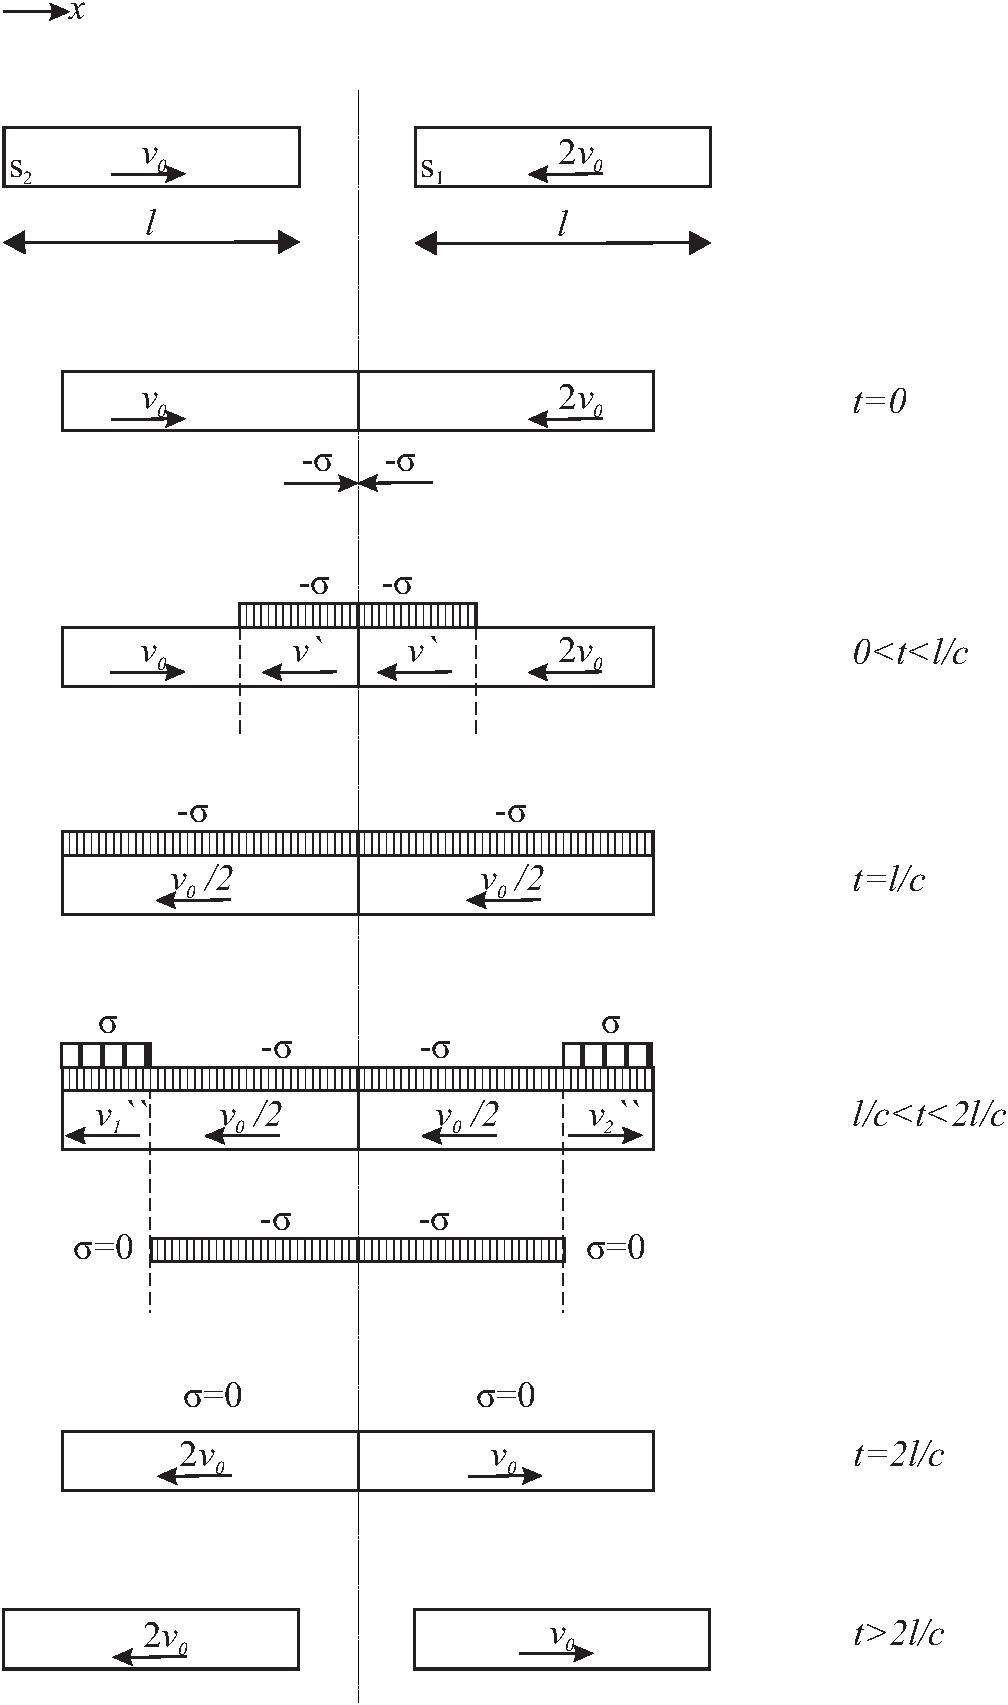
\includegraphics[width = 0.8\textwidth ]{figures/impact_of_two_bars.pdf}
    \caption{Different steps in the impact of two identical bars with different initial velocities.}
    \label{fig:p1}
\end{figure}


% \newpage
% \bibliography{ref}
% \bibliographystyle{ieeetr}

\end{document}